%
% -- Manlio Modugno

\documentclass{beamer} 
\usepackage{eulervm}
%\usepackage{booktabs}
\usepackage{listings}
\usepackage{bold-extra}
\usepackage{cancel}
\usepackage{fancybox}
\usepackage{soul}
\usepackage[english]{babel}
\usepackage[utf8]{inputenc}
\usepackage{hyperref}
\usepackage{amsmath}
%\hypersetup{colorlinks=true,urlcolor=blue}

\newcommand{\codefont}{\fontsize{6}{8}\selectfont}
\lstset{language=[Sharp]C, 
captionpos=b, 
frame=lines,
lineskip= 1pt, %space between lines
basicstyle=\codefont, 
keywordstyle=\color{blue}, 
commentstyle=\color{green}, 
stringstyle=\color{red}, 
numbers=left, 
numberstyle=\tiny, 
stepnumber=2,
numbersep=5pt,
breaklines=true, 
breakatwhitespace=false,
showstringspaces=false,
frame=single,
tabsize=2,
emph={double,bool,int,unsigned,char,true,false,void},
emphstyle=\color{blue},
emph={Assert,Test},
emphstyle=\color{red},
emph={[2]\using,\#define,\#ifdef,\#endif},
emphstyle={[2]\color{blue}}
}


\mode<presentation>
\definecolor{title_color}{RGB}{2,128,181} 
\usetheme{Ilmenau}
\usecolortheme[named=title_color]{structure}
\setbeamercolor{palette quaternary}{use=structure,fg=black,bg=white} %header footer color
\useoutertheme[subsection=false]{smoothbars}
\setbeamercovered{transparent}
\setbeamertemplate{navigation symbols}{}
\setbeamerfont{subsection in toc}{size=\scriptsize}

\title{Sequence Diagram + Refactoring chapter 1}
\author{Manlio Modugno}
\institute[GMTechnologies] 

\date[30.06.2016] 
{30.06.2016 - Sequence Diagram + Refactoring chapter 1}

\subject{}

\graphicspath{{img/}}
\pgfdeclareimage[height=0.6cm]{mfg-logo}{img/mfgLogo}
\logo{\pgfuseimage{mfg-logo}}

%
% Content start
%
\begin{document}
\begin{frame}
  \titlepage
\end{frame}

\begin{frame}
  \frametitle{Argomenti Trattati}
  \tableofcontents
\end{frame}

\section{Sequence Diagram}
\subsection{Basics}
\begin{frame}
  \frametitle{Basics}
  \begin{itemize}
  		\item<+-> Define event sequences that result in some desired outcome
		\item<+-> Focus is on the order in which messages occur
		\item<+-> Vertical dimension: shows (top down) the time sequence of messages
		\item<+-> Horizontal dimension: shows (left right) the objects involved in the messages communication
  \end{itemize}
\end{frame}

\subsection{Lifeline}
\begin{frame}
	\frametitle{Lifeline}
	\begin{center}
		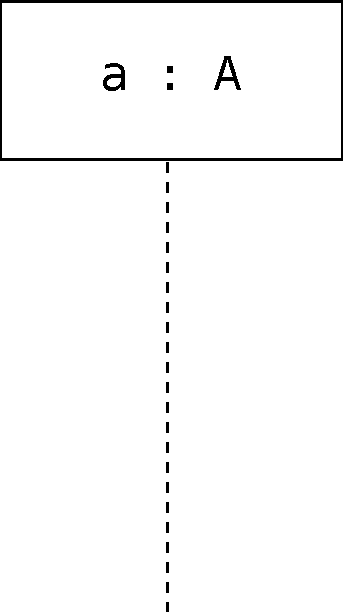
\includegraphics[scale=0.4]{box}
	\end{center}
	\textbf{Note:}
	\begin{itemize}
  			\item Drown as a box with a dashed line.
  			\item Name is inside the box  $\Rightarrow$ instance/role name [optional] : Class Name
  			\item Instances are underlined, role not.
	\end{itemize}
\end{frame}

\subsection{Messages}
\begin{frame}
	\frametitle{Messages}
	\begin{center}
		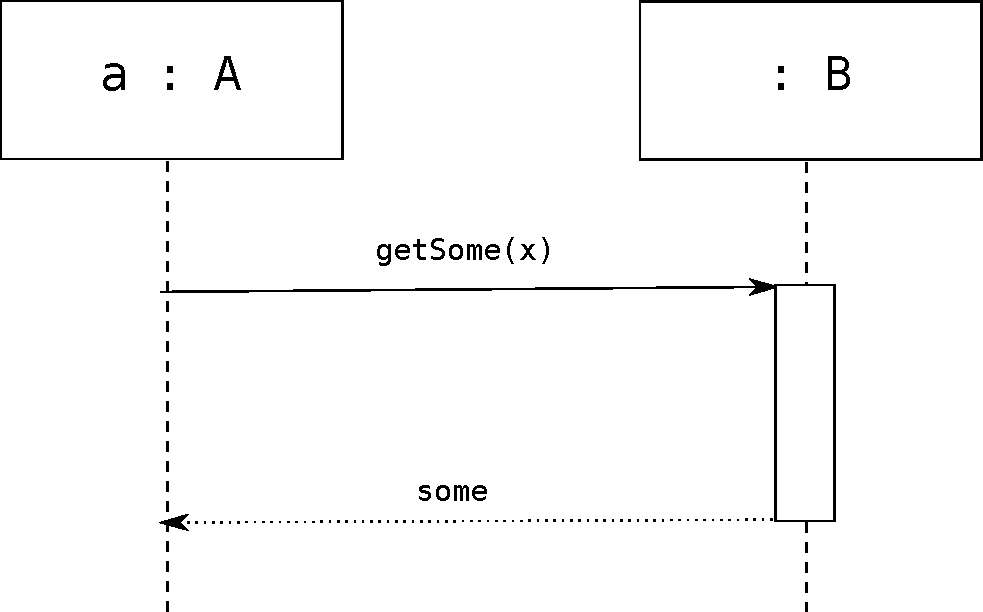
\includegraphics[scale=0.35]{messages}
	\end{center}
	\textbf{Note:}
	\begin{itemize}
  			\item Messages depicted as arrowhead lines 
  			\item Message name placed above the arrowed line
  			\item Message sent on a receiving object is a method that the receiving object's class implements.
  			\item Dotted arrowhead represent return value [optional]
	\end{itemize}
\end{frame}

\subsection{Guards}
\begin{frame}
	\frametitle{Guards}
	\begin{center}
		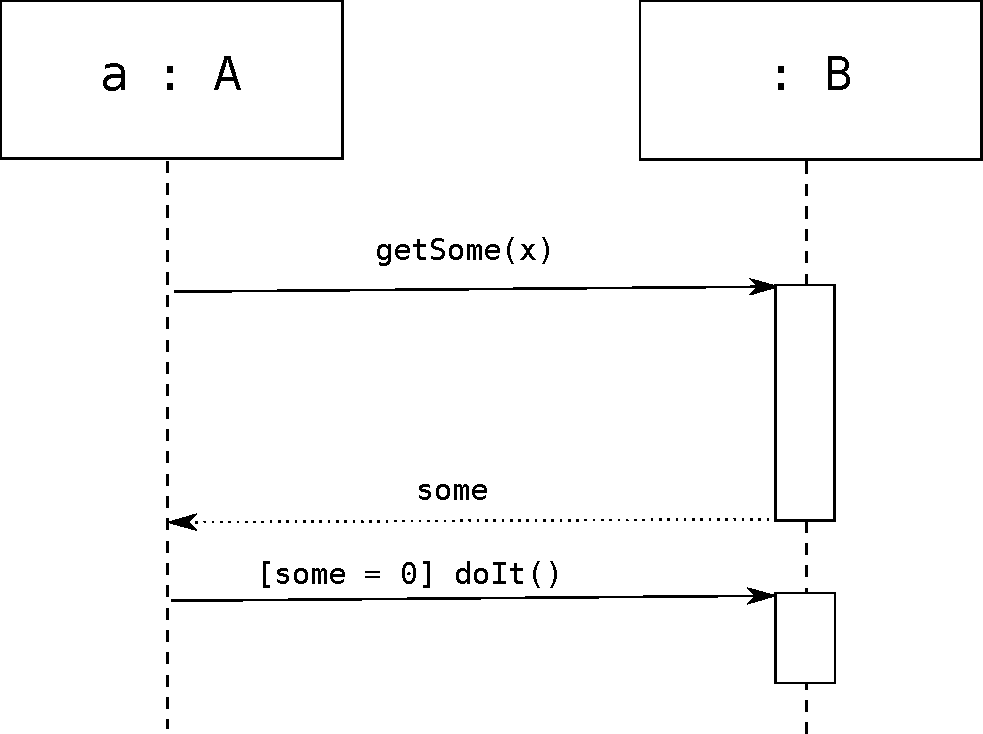
\includegraphics[scale=0.35]{guards}
	\end{center}
	\textbf{Note:}
	\begin{itemize}
  			\item When a condition must be met for a message to be sent
  			\item If some = 0 doIt() message is sent to B
	\end{itemize}
\end{frame}

\subsection{Combined fragments}
\begin{frame}
	\frametitle{Combined fragments: alternatives / options / loops}
	\begin{center}
		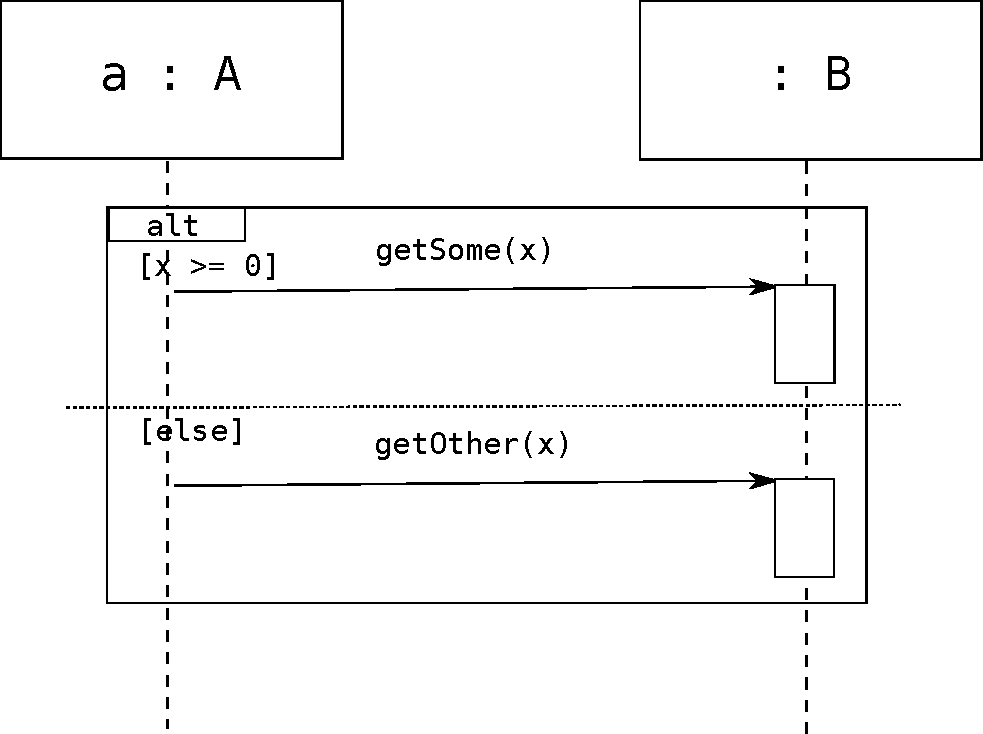
\includegraphics[scale=0.25]{alt}
	\end{center}
	\textbf{Note:}
	\begin{itemize}
  			\item Used to group sets of messaged together to show conditional flow
  			\item \textbf{Alternatives:} models if then else conditional with label ``alt'' and optional guards
  			\item \textbf{Options:} models if then conditional with label ``opt''
  			\item \textbf{Loops:} models a repetitive sequence with label ``loop'' and optional guard
	\end{itemize}
\end{frame}
\end{document}